% Author Thomas C. Hales
% Copyright Thomas C. Hales
% Format latex.
% 

%!TEX TS-program = latex    
%% This line is for TexShop. 

% Revision history. See svn.
% Jan 24, 2009

\documentclass[cup9a]{cupbook}
%% Cambridge University Press Macros from
%% https://authornet.cambridge.org/information/productionguide/laTex_files/

%

\usepackage{graphicx}
\usepackage{verbatim}
\usepackage{latexsym}
\usepackage{amsfonts}
\usepackage{amsmath}
\usepackage{makeidx}
\usepackage{multicol}
\usepackage{crop}
\usepackage{txfonts}
%\usepackage{pdfsync}  %for TexShop sync.
\usepackage[letterpaper,colorlinks=true,
            ps2pdf,hyperindex=true]{hyperref}
%\usepackage{mparhack} %http://www.tex.ac.uk/cgi-bin/texfaq2html?label=marginparside
\usepackage{multind}


 
%-%
% --Repository--
%-%
% generate revision number by
% svn propset svn:keywords "LastChangedRevision" macros.tex
\def\svninfo{%
  TeXed on \today; \hfill\break
  Repository Root: https://flyspeck.googlecode.com/svn \hfill\break
  SVN $LastChangedRevision$
  }

%-%
% --Graphics--
%-%
%set \showgraphics option in flag_fly.tex
% flypaper graphics
\def\myincludegraphics#1{%
      \if\showgraphics t{\includegraphics{#1}}%
      \else{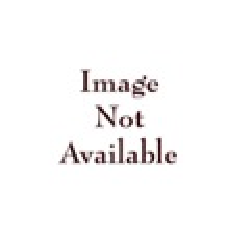
\includegraphics{noimage.eps}}\fi}

%-%
% --Footnotes--
%-%
% http://help-csli.stanford.edu/tex/latex-footnotes.shtml
\long\def\symbolfootnote[#1]#2{\begingroup%
\def\thefootnote{\ensuremath{\fnsymbol{footnote}}}\footnote[#1]{#2}\endgroup}

%-%
% --Special Formatting--
%-%
% http://en.wikibooks.org/wiki/LaTeX/Formatting#List_Structures
\renewcommand{\labelitemii}{$\star$}

%-%
% --Symbols--
%-%
\def\sland{\ \land\ }

% brackets
\def\leftopen{]}
\def\leftclosed{[}
\def\rightopen{[}
\def\rightclosed{]}

% squiqqly relations
\def\seq{\approx}
\def\sle{\preceq}
\def\sge{\succeq}
\def\slt{\prec}
\def\sgt{\succ}

% mathbb
\def\R{{\mathbb R}}
\def\N{{\mathbb N}}
\newcommand{\ring}[1]{\mathbb{#1}}
\def\A{{\mathbf A}}
\def\Rp{\ring{R}^{3\,\prime}}

% operatorname
\def\op#1{{\operatorname{#1}}}
\def\optt#1{{\operatorname{{\texttt{#1}}}}}

% color
\definecolor{LightBlue}{rgb}{0.3,0.3,1.0}
\definecolor{RawSienna}{rgb}{0.5,0.04,0.2}
\def\hc#1{\textcolor{RawSienna}{#1}}
\def\mc#1{\textcolor{LightBlue}{#1}}

\def\fst{\op{fst}}
\def\snd{\op{snd}}


%%
%\makeindex{guid}

 \crop
%\makeindex



% CUP BOOK CLASS SPECIFIC
\newtheorem{lemma}{Lemma}[chapter]
\newtheorem{definition}{Definition}[chapter]
\newtheorem{remark}{Remark}[chapter]
\newtheorem{theorem}{Theorem}[chapter]
\newtheorem{corollary}{Corollary}[chapter]
\newtheorem{example}{Example}[chapter]
\newtheorem{claim}{Claim}[chapter]
\newtheorem{notation}{Notation}[chapter]
\newtheorem{assumption}{Assumption}[chapter]
\newtheorem{interpretation}{Interpretation}[chapter]

%%%%%%%%%%%%%%%%%%%%%%%%%%%%%%%%%%%%%%%%%%%%%%%%%%%%

\begin{document}
\raggedbottom  % for now.
%\raggedright  % don't worry for now.

    \title{The Foundations of Mathematics :
      %\\ \phantom{Hello}
      \\  An Introductory Course in Higher Order Logic}
    \author{Thomas C. Hales}
    \maketitle
    \frontmatter
    \tableofcontents
    \thanks

\mainmatter

\noindent

\bigskip\noindent
This material is based upon work supported by the National Science
Foundation under
Grants 0503447 and 0804189.

\bigskip\noindent\svninfo 

%\bigskip\noindent
%A pdf of an earlier version of this work appears at\hfill\break 
%\url{http://www.math.pitt.edu/~thales/papers/Flyspeck_Blueprint_2008.pdf}.

\bigskip\noindent
%% XX Thanks to Tran Nam Trung on the hypermap chapter.

%% INDEX OF FORMAL TERMS.

\def\idx#1#2{\indy{Spec}{{\tt #1}; #2}}
\def\idz#1#2#3{\indy{Spec}{{\tt #1}; #2; {\tt \textbackslash \string#3}}}
\idx{pt}{$\pt$}
\idz{atn2~x~~y}{$\atn(x,y)$}{atn}
\idx{sqrt8}{$\sqrt8$}
\idx{sqrt2}{$\sqrt2$}
\idx{t0}{$t_0$}
\idx{two\_t0}{$2t_0$}
\idx{square\_2t0}{$(2t_0)^2$}
\idx{square\_4t0}{$(4t_0)^2$}
\idx{zeta}{$\zeta$}
\idz{doct}{$\doct$}{doct}
\idz{dtet}{$\dtet$}{dtet}
\idx{pi\_rt18}{$\pi/\sqrt{18}$}
\idx{rogers}{$\sqrt2/\zeta$}
\idx{compression\_cut}{$1.41$}
\idz{squander\_target}{$\squander$}{squander}
\idz{xi\_gamma}{$\xiG$}{xiG}
\idz{xiV}{$\xiV$}{xiV}
\idx{xi'\_gamma}{$\xiG'$}
\idz{xi\_kappa}{$\xik$}{xik}
\idz{xi\_kappa\_gamma}{$\xikG$}{xikG}
\idz{pi\_max}{$\maxpi$}{maxpi}
\idx{t4}{$t_4$}
\idx{t5}{$t_5$}
\idx{t6}{$t_6$}
\idx{t7}{$t_7$}
\idx{t8}{$t_8$}
\idx{t9}{$t_9$}
\idx{t10}{$t_{10}$}
\idx{s5}{$s_5$}
\idx{s6}{$s_6$}
\idx{s7}{$s_7$}
\idx{s8}{$s_8$}
\idx{s9}{$s_9$}
\idx{s10}{$s_{10}$}
\idx{eps0}{$\epsilon_0$}
\idx{Z31}{$Z_{3,1}$}
\idx{D31}{$D_{3,1}$}
\idx{Z31}{$Z(\y{(3,1)})$}
\idx{Z32}{$Z(\y{(3,2)})$}
\idx{Z33}{$Z(\y{(3,3)})$}
\idx{Z41}{$Z(\y{(4,1)})$}
\idx{Z42}{$Z(\y{(4,2)})$}
\idx{D31}{$D(\y{(3,1)})$}
\idx{D32}{$D(\y{(3,2)})$}
\idx{D33}{$D(\y{(3,3)})$}
\idx{D41}{$D(\y{(4,1)})$}
\idx{D42}{$D(\y{(4,2)})$}
\idx{D51}{$D(\y{(5,1)})$}
\idz{delta\_x x1 ... }{$\Delta(x_1,\ldots)$}{Delta}
\idx{delta\_x4 x1 ... }{$\Delta_4(x_1,\ldots)$}
\idx{delta\_x6 x1 ... }{$\Delta_6(x_1,\ldots)$}
\idz{ups\_x x1 ...}{$\ups(x_1,\ldots)$}{ups}
\idz{eta\_x x1 x2 x3}{$\eta(\sqrt{x_1},\sqrt{x_2},\sqrt{x_3})$}{eta}
\idz{eta\_y y1 y2 y3}{$\eta(y_1,y_2,y_3)$}{eta}
\idz{rho\_x x1 ... }{$\rho(x_1,\ldots)$}{rho}
\idx{rad2\_y y1 ... }{$(\rad_V\{v_0,v_1,v_2,v_3\})^2,\ y_1 = |v_0-v_1|,\ldots$}
\idz{chi\_x x1 ... }{$\chi(x_1\ldots)$}{chi}
\idz{dih\_x x1 ... }{$\dih(\sqrt{x_1},\ldots)$}{dih}
\idz{dih\_y y1 ... }{$\dih(y_1,\ldots)$}{dih}
\idx{dih2\_x x1 x2 ... }{$\dih(\sqrt{x_2},\ldots)$}
\idx{dih2\_y x1 x2 ... }{$\dih(y_2,\ldots)$}
\idx{dih3\_x x1 x2 ... }{$\dih(\sqrt{x_3},\ldots)$}
\idx{dih3\_y x1 x2 ... }{$\dih(y_3,\ldots)$}
\idz{sol\_x x1 ... }{$\sol(v_0,\ldots),\ x_1=|v_0-v_1|^2,\ldots$}{sol}
\idz{sol\_y y1 ... }{$\sol(v_0,\ldots),\ y_1=|v_0-v_1|,\ldots$}{sol}
\idx{vol\_x x1 ... }{$\sqrt{\Delta(x_1,\ldots)}/12$}
\idz{beta psi theta}{$\beta_\psi\theta$}{beta}
\idz{arclength a b c}{$\arc(a,b,c)$}{arc}
\idx{volR a b c}{$\op{volR}(a,b,c)$}
\idx{solR a b c}{$\op{solR}(a,b,c)$}
\idx{dihR a b c}{$\op{dihR}(a,b,c)$}
\idx{vorR a b c}{$\op{sovoR}(a,b,c,\lambda_{oct})$}
\idx{denR a b c}{$\delta(a,b,c)$}
\idx{tauR a b c}{$\op{sovoR}(a,b,c,\lambda_{sq})$}
\idx{qy y1 y2 y3 t}{$\op{quovol}(a,b,c)$}
\idx{quo\_x x y z}{}
\idx{qn y1 y2 z t}{}
\idx{phi h t}{}
\idx{phi0}{}
\idx{eta0 h}{}
\idx{crown h}{}
\idx{anc y1 y2 y6}{}
\idx{K0 y1 y2 y6}{}
\idx{AH h t}{}
\idx{BHY y}{}
\idx{KY y1 y2 y3 y4 y5 y6}{}
\idx{KX x1 x2 x3 x4 x5 x6}{}
\idx{vor\_analytic\_x x1 x2 x3 x4 x5 x6}{}
\idx{vor\_analytic\_x\_flipped x1 x2 x3 x4 x5 x6}{}
\idx{octavor\_analytic\_x x1 x2 x3 x4 x5 x6}{}
\idx{tau\_analytic\_x x1 x2 x3 x4 x5 x6}{}
\idx{kappa y1 y2 y3 y4 y5 y6}{}
\idx{kappa\_dih\_y y1 y2 y3 y5 y6 d}{}
\idx{level\_at h t}{}
\idx{vorstar h1 h2 h3 a1 a2 a3 t}{}
\idx{vort\_y y1 y2 y3 y4 y5 y6 t}{}
\idx{vor\_0\_y y1 y2 y3 y4 y5 y6}{}
\idx{tau\_0\_y y1 y2 y3 y4 y5 y6}{}
\idx{vor\_0\_x x1 x2 x3 x4 x5 x6}{}
\idx{tau\_0\_x x1 x2 x3 x4 x5 x6}{}
\idx{vort\_x x1 x2 x3 x4 x5 x6 t}{}
\idx{tauVt\_x x1 x2 x3 x4 x5 x6 t}{}
\idx{vorA\_x x1 x2 x3 x4 x5 x6}{}
\idx{tauA\_x x1 x2 x3 x4 x5 x6}{}
\idx{vorC0\_x x1 x2 x3 x4 x5 x6}{}
\idx{tauC0\_x x1 x2 x3 x4 x5 x6}{}
\idx{vorC\_x x1 x2 x3 x4 x5 x6}{}
\idx{tauC\_x x1 x2 x3 x4 x5 x6}{}
\idx{v0x x1 x2 x3 x4 x5 x6}{}
\idx{v1x x1 x2 x3 x4 x5 x6}{}
\idx{gamma\_x x1 x2 x3 x4 x5 x6}{}
\idx{tau\_gamma\_x x1 x2 x3 x4 x5 x6}{}
\idx{rad2\_x x1 x2 x3 x4 x5 x6}{}
\idx{sigma\_qrtet\_x x1 x2 x3 x4 x5 x6}{}
\idx{sigma1\_qrtet\_x x1 x2 x3 x4 x5 x6}{}
\idx{tau\_sigma\_x x1 x2 x3 x4 x5 x6}{}
\idx{sigma32\_qrtet\_x x1 x2 x3 x4 x5 x6}{}
\idx{mu\_flat\_x x1 x2 x3 x4 x5 x6}{}
\idx{taumu\_flat\_x x1 x2 x3 x4 x5 x6}{}
\idx{mu\_upright\_x x1 x2 x3 x4 x5 x6}{}
\idx{mu\_flipped\_x x1 x2 x3 x4 x5 x6}{}
\idx{vor\_0\_x\_flipped x1 x2 x3 x4 x5 x6}{}
\idx{octavor0\_x x1 x2 x3 x4 x5 x6}{}
\idx{nu\_x x1 x2 x3 x4 x5 x6}{}
\idx{nu\_gamma\_x x1 x2 x3 x4 x5 x6}{}
\idx{taunu\_x x1 x2 x3 x4 x5 x6}{}
\idx{octa\_x x1 x2 x3 x4 x5 x6}{}
\idx{sigmahat\_x x1 x2 x3 x4 x5 x6}{}
\idx{sigmahat\_x' x1 x2 x3 x4 x5 x6}{}
\idx{sigmahatpi\_x x1 x2 x3 x4 x5 x6}{}
\idx{tauhat\_x x1 x2 x3 x4 x5 x6}{}
\idx{tauhatpi\_x x1 x2 x3 x4 x5 x6}{}
\idx{pi\_prime\_tau k0 k1 k2}{}
\idx{pi\_prime\_sigma k0 k1 k2}{}



  % Formal Spec Index.

\smallskip
\newpage



%%%%%%%%%%%%%%%%%%%%%%%%%%%%%%%%%%%%%%%%%%%%%%%%%%%%


%%  \label{part:intro}
   \newpage

   \setcounter{chapter}{-1}
   \chapter{Preface}
   \label{XX}  % for missing references. XX.

   

\end{document}
